\documentclass{article}

% if you need to pass options to natbib, use, e.g.:
%     \PassOptionsToPackage{numbers, compress}{natbib}
% before loading neurips_2019

% ready for submission
% \usepackage{neurips_2019}

% to compile a preprint version, e.g., for submission to arXiv, add add the
% [preprint] option:
\usepackage[preprint]{neurips_2019}
\bibliographystyle{unsrt}

% to compile a camera-ready version, add the [final] option, e.g.:
%     \usepackage[final]{neurips_2019}

% to avoid loading the natbib package, add option nonatbibnatbib:
%     \usepackage[nonatbib]{neurips_2019}

\usepackage[utf8]{inputenc} % allow utf-8 input
\usepackage[T1]{fontenc}    % use 8-bit T1 fonts
\usepackage{hyperref}       % hyperlinks
\usepackage{url}            % simple URL typesetting
\usepackage{booktabs}       % professional-quality tables
\usepackage{amsfonts}       % blackboard math symbols
\usepackage{nicefrac}       % compact symbols for 1/2, etc.
\usepackage{microtype}      % microtypography
\usepackage{graphicx}
\usepackage{titlesec}
\usepackage{hyperref}
\usepackage{enumitem}
\usepackage{lmodern}
\usepackage{amsmath}
\usepackage{fancyhdr}
\usepackage{textcomp}
\usepackage{lmodern}% http://ctan.org/pkg/lm
\usepackage[table,x11names,svgnames]{xcolor}
\usepackage{soul}
\usepackage{parskip}
\usepackage{multirow}
\usepackage{array}
\usepackage{afterpage}
\usepackage{tabularx}
\usepackage{float}
\usepackage{placeins}
\usepackage{tablefootnote}
\usepackage{microtype}
\usepackage{textcomp}
\usepackage{titlesec}
\usepackage{enumitem}
\usepackage{listings}
\usepackage{subcaption}
\usepackage{verbatim}
\usepackage[htt]{hyphenat}
\usepackage[linesnumbered, noline, noend]{algorithm2e}

% optimization
\DeclareMathOperator*{\argmin}{arg\,min}
\DeclareMathOperator*{\argmax}{arg\,max}


\title{Learn to play Go}

\author{%
  Albert Liu \\
  Department of Computer Science\\
  Stanford University\\
  \texttt{albertpl@stanford.edu} \\
}

\begin{document}

\maketitle

\section{Introduction}

The ancient Chinese game of Go is considered the hardest classic board game and until recently it had been a grand challenge for AI. It has relatively simple rules but vast possibilities of strategies, which typically requires decades of study to master.  Recently AlphaGo \cite{silver2016mastering}, AlphaGoZero \cite{silver2017masteringalphagozero} and AlphaZero \cite{silver2017masteringalphazero}, developed by a DeepMind team, has rocked the world of AI and Go by soundly beating the best Go human players in the world.

The goal of this project is to train a agent that can win games against our oracle without incorporating lots of domain knowledge of the game. We formulate Go as a turn-taking, two player, zero-sum game of perfect information. The state space is 8 recent boards of possible placements of the stones and the player who plays that turn, represented as either black stone or white stone. The state is fully observable as input. The action space is any legal position of a stone, given the current state, and a pass action. We set the reward to +1 if current player wins, -1 if loses. No reward otherwise. Figure \ref{fig:goboard} shows a concrete Go board and white stone is making a move at $P15$. 

Generic search methods, such as Minimax search, are intractable due to enormous search space $(\sim 10^{170})$ and large number of legal move per state$(\sim 250)$. The other challenge comes from the need for massive computational resources. For example, AlphaGoZero use 64 GPUs and 19 CPUs to play 5 millions games to achieve superhuman level \cite{silver2017masteringalphagozero}.

\section{Related Work}
Monte Carlo Tree Search (MCTS) is a common ingredient for most of recent Go programs. Browne \textit{et al.} gives a great survey on MCTS \cite{browne2012survey}. Kocsis \textit{et al.} develops Upper Confidence Tree \cite{kocsis2006bandit} algorithm by applying UCB1 \cite{auer2002finite} as tree policy, which greatly improves the state of the art for Go programs. There are various improvements. RAVE \cite{gelly2007combining} distributes the updated values of the simulation results to larger set of nodes than the sampled path from root to the leaf. And it applies AMAF \cite{bouzy2004monte} (all-move-as-first), which keep previous simulations and apply it whenever we examine the same $(s, a)$ edge and then combines it with regular simulations.

Deep Neural Network (DNN), especially Convolutional Neural Network, has been used to predict the next move and as the basis for strong Go program, such as \cite{tian2015better} and \cite{maddison2014move}. The first Go program that defeats top professional player is AlphaGo \cite{silver2016mastering}, which combines DNN, supervised learning, MCTS and reinforcement learning. Subsequently, the same DeepMind team develops AlphaGoZero\cite{silver2017masteringalphagozero} without human data or guidance beyond the game rules, which learned exclusively through self-play reinforcement learning. Then they generalize it to more diverse game setting and build AlphaZero \cite{silver2017masteringalphazero}.

\section{Dataset and Environment}

We collect experiences (i.e. game records) for our reinforcement learning based approaches. The standard approach is to have agents play against themselves through simulated games, i.e. self-play. We record the board position at each step,  the move, the final reward ( +1 for win and -1 for loss) and network outputs from current player's perspective. 

As illustrated in Figure \ref{fig:env}, our simulator includes a Go gameplay engine, which is based on Pachi \cite{baudivs2011pachi}, an open source Go framework, and parts of the environment is adopted from OpenAI gym \cite{brockman2016openai}. We choose Pachi mainly because of the optimal gameplay time. For each player, the input is a 2D numpy array (e.g. $9 \times 9$), representing current board with each element encoding the color of stone, 0 for empty, 1 for black stone and 2 for white stone. The output of each player is the next move to play, which is a scalar that either represents encoded board position (e.g. 50 represents "E4") or a pass action (e.g. 81). Each player can optionally persist the game records, i.e. numpy arrays that hold the board representation, moves and etc., to disk, which are used as experiences for further reinforcement learning. We use Keras \cite{chollet2015keras} as our deep learning framework. 

\section{Methods}
We restrict our attention to $9 \times 9$ board because of resources limitation. Minimax search or AlphaBeta pruning, however, is still intractable. Instead, we start with UCT \cite{kocsis2006bandit}. Then we will explore policy gradient based methods. Finally we will combine tree search and function approximation approach, following AlphaGoZero \cite{silver2017masteringalphagozero}.  But first, we discuss the baseline and oracle.

\subsection{Baseline}
For baseline, we write a random player which selects legal move randomly, except that it won't commit suicide, i.e. filling in its own eye, which is an empty position where all adjacent positions and three out of four diagonally adjacent positions are its stones (or edges).

\subsection{Oracle}
We use Pachi built-in \textit{UCT} engine as our oracle which is said to achieve highest amateur expect level (KGS 7 dan) on $9 \times 9$ board with reasonable hardware, where dan is expert Go ranking, from 1 to 7 (low to high). Technically the \textit{UCT} engine implements RAVE \cite{gelly2007combining}, instead of classic UCT. This engine incorporates lots of heuristics and $3 \times 3$ pattern, e.g. self-atari detector and ladder testing \cite{baudivs2011pachi}.

\subsection{Monte Carlo Tree Search}
\label{sec:mcts}

\begin{figure}[H]
\centering
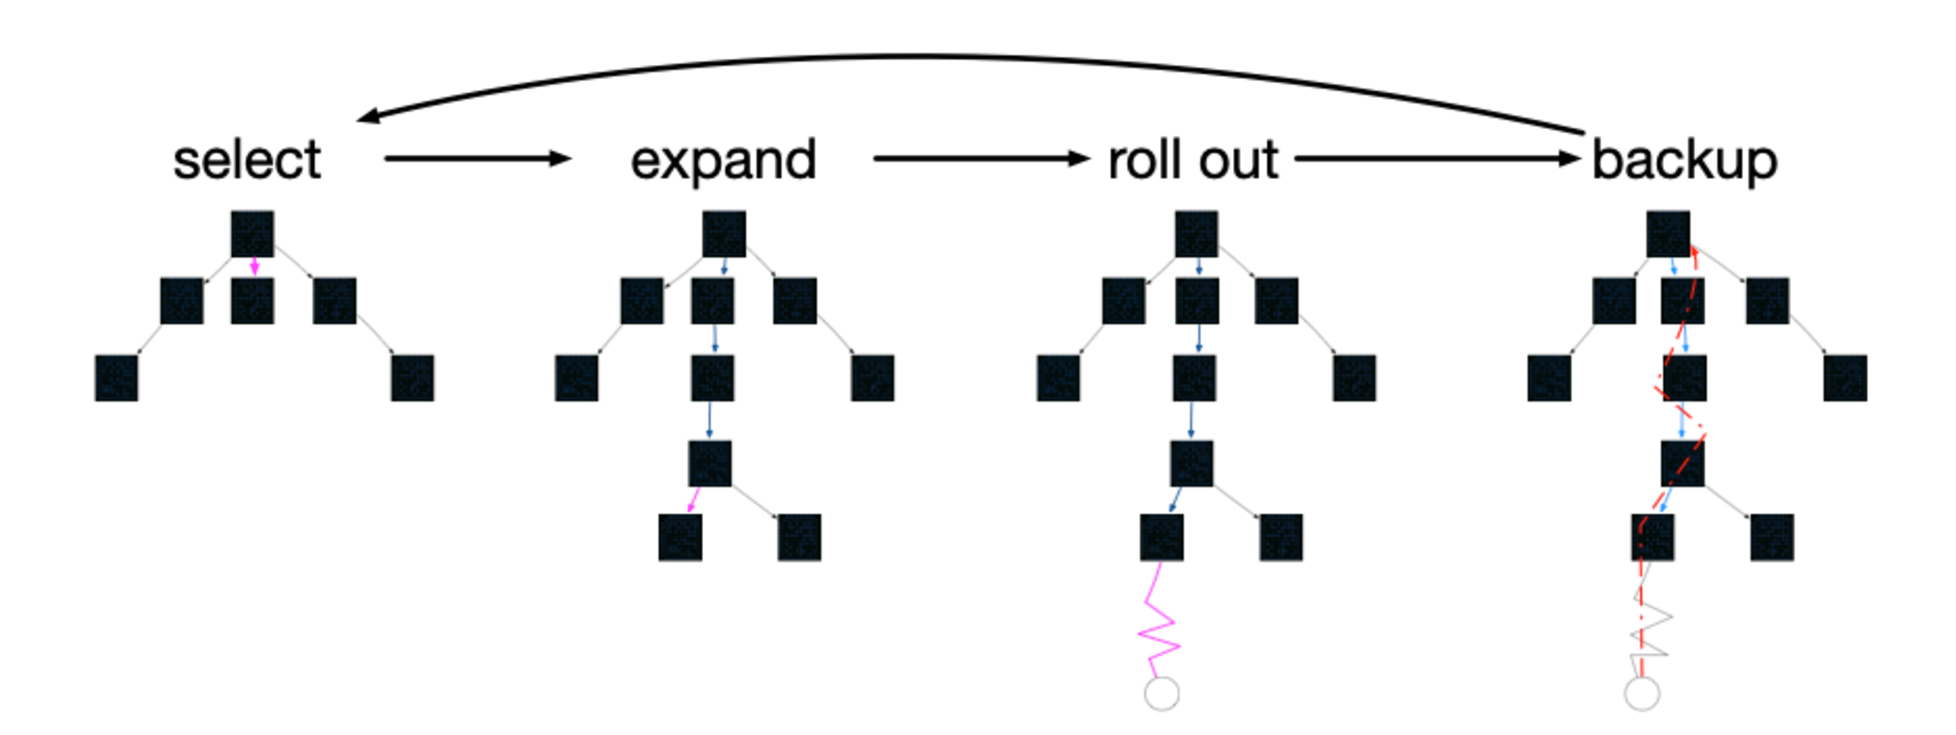
\includegraphics[width=0.5\linewidth]{mcts}
\caption{MCTS}
\label{fig:mcts}
\end{figure}

We apply MCTS approach to the game of Go. Each node of the search tree is a game state, which is tuple of board representation and player to play. And there is an edge between node $s$ and node $s'$ if and only if there exists some move $a$ such that $s' = \text{Succ}(s, a)$, where $\text{Succ}(s,a)$ is function that returns the next game state $s'$, which is the alternated player and a new board produced by playing the move $a$ on the board of $s$. For each  $s, a$, we maintain visit count $n(s,a)$ and value $q(s,a)$. 

As described in Algorithm \ref{algo:mcts}, when player is asked to make a move, it create a new tree with current game state $s_0$ as the root node. Then the player simulates multiple random games (each is called a rollout) to evaluate the moves. For each rollout, initially it follows tree policy to traverse the tree down and then expands new node once it reaches the leaf of the tree. From the newly expanded node, it will follow a rollout policy (we use random policy) to finish the game. The final reward is backed up to all the nodes along the path back to root node. Once all rollouts are done, the player selects the move with the maximum visit counts from the root node. 

\begin{algorithm} 
  \DontPrintSemicolon
  \caption{MCTS with UCB policy}
  \label{algo:mcts}
  \KwIn{root node $s_0$: current game state}
  \KwIn{$c>0$: parameter to control the degree of exploration}
  \While {within computation bound} {
    $ s \gets s_0 $ \\
    $ \Delta \gets \emptyset$ \\
    // selection based on tree policy, e.g. UCB1 \cite{auer2002finite} \\
    \While {$s$ is in the tree} {
      $a  \gets \argmax \{ q(s, a) + c \sqrt{\frac{\log \sum_{a'}n(s, a')}{n(s,a)}}$ \}\\
      $\Delta \gets \Delta \cup \{(s, a)\}  $ \\
      $s \gets \text{Succ}(s, a) $\\
    }
    expand tree with the new node $s$ \\
    continue the game from $s$ with random policy and let $r$ be the reward \\
    // update each node on the path $s_0 \rightarrow ... \rightarrow s$ \\
    \For {$s, a \in \Delta $ } {
      $ n(s, a) \gets n(s,a) + 1 $ \\
      $ q(s, a) \gets q(s,a) +  \frac{1}{n(s,a)} (r - q(s,a))$ \\
    }
  }
  \Return{$\argmax_{a} q(s_0, a) $}
\end{algorithm}

Figures \ref{fig:mctsselect}, \ref{fig:mctsexpand}, \ref{fig:mctsbackup}, \ref{fig:mctsfinal} show concret examples for each MCTS step.

\subsubsection{Other techniques}
\label{sec:othertechniques}
To increase exploration, we follow \cite{silver2017masteringalphagozero} and apply these techniques
\begin{itemize}
  \item
    The second term in UCB1 can be viewed as uniform priors on uncertainty. Additional Dirichlet noise can be added to it, $ (1-\epsilon) \text{Uniform}(s,a) + \epsilon \eta_a$ and $\eta \sim \text{Dirichlet}(\delta)$
  \item 
  Instead of greedy selection after each tree search, we select the action proportionally to the visit counts for the first $\gamma$ moves of the games which allows more diverse moves at the beginning of the games. For the rest of the game, we switch back to greedy selection.
\end{itemize}
Both $\delta, \gamma$ are considered hyperparameters for our MCTS algorithm.


\subsection{REINFORCE with baseline}
The policy gradient based methods, such as REINFORCEMENT \cite{williams1987reinforcement}, allow us to learn stochastic policy naturally, compared to using $\epsilon-$ greedy policy in Q-learning. REINFORCE method uses Monte Carlo method to sample return to compute an unbiased estimation of the gradient. But typically Monte Carlo methods have high variance and therefore produces slow learning. An extra baseline term, as suggested in \cite{sutton2018reinforcement}, can greatly reduce the variance without any bias, because the added term has an expectation of zero. We now describe how we apply this method in this problem.


\subsubsection{Network architecture}
\label{sec:nn}
Let $t$ be current move index of current player, $S_t$ be state the player makes decision on and $A_t$ be move the player will take. As shown in Figure \ref{fig:nn}, we have a two headed deep neural network to approximate both the policy function $\pi_{\theta}(A_t|S_t)$ and state value function $v_w(S_t)$.  The input to this network is $S_t$, which is an binary array in the shape of $17 \times 9 \times 9$, where $9$ is the board size and $17$ is the number of channels and each channel is described as following 

\begin{enumerate}
  \item
    For $i = 0, ..., 7$, channel $i$ is a $9 \times 9$ 2D array and each element is an indicator if current player has a stone at the position, at time $t-i$.
  \item
    For $j = 0, ..., 7$, channel $j+8$ is a $9 \times 9$ 2D array and each element is an indicator if opponent player has a stone at the position, at time $t-j$.
  \item
    The last channel ($16$) encodes current player, 1 for black player and 0 for white player.
\end{enumerate}
The history of the board is necessary because \textit{Ko} (repetition is restricted) is not directly observable otherwise.

The outputs of the network are 
\begin{itemize}
  \item
    $\pi_{\theta} (A_t|S_t)$

    A $82$-tuple of representing the probability vector for taking each action $A_t$ for $S_t$ for current player. The action space size is $9 ^2 + 1 = 82$.

  \item
    $v_w(S_t)$

    A scalar between -1 and +1, representing the predicated value for $S_t$, from the perspective of current player.

    Figure \ref{fig:inference} shows an sample input/output for the neural network.
\end{itemize}

$\theta$ and $w$ share most of the parameters (ResNet and two Fully Connected layers), except that $\theta$ includes a Softmax layer and $w$ includes a Tanh layer.

The network architecture is similar to what is used in \cite{silver2017masteringalphagozero}, except that we use shorter residual tower with less convolution filters.  Table \ref{tbl:nna} describes the architecture in details.


\subsubsection{Training procedure}
We update parameters $\theta$ and $w$ continuously through last 10 games gathered through self-play.  Let $\alpha$ be the learning rate,  $G_t$ be return. Let $s_t, a_t, r_t$ be specific training sample, representing player taking action $a_t$ at state $s_t$ and yielding final reward $r_t$.

For policy function and $\theta$. The objective function is  $J(\theta) = V_{\pi_{\theta}}(S_t)$ and update rule is
$$ \theta_{t+1} = \theta_{t} + \alpha 
( r_t  - v_w(s_t))
\nabla_{\theta} \log \pi_{\theta}(a_t|s_t) 
$$

For value function and $w$. The objective function is  $J(w) = ||v_w(S_t) - G_t||^2$ and update rule is 
$$ w_{t+1} = w_{t} + \alpha 
( r_t  - v_w(s_t))
\nabla_{w} v_w(s_t) 
$$
\subsection{Combination of tree search and DNN}
\label{sec:combined}
Finally we will combine MCTS and function approximation with DNN, in the same way as in \cite{silver2017masteringalphagozero}. This method can be viewed as an general form of policy iteration \cite{sutton2018reinforcement}. And we reuse the same DNN as described in \ref{sec:nn}. We repeat the following two steps until it converges

\begin{itemize}
  \item
    Self play with DNN guided tree search

    We use self play to gather experiences. The tree search is augmented by the DNN in the following way
    \begin{itemize}
   \item
    whenever we expand a new node $s$, instead of playing out the rest of the game to estimate the value, we perform an inference over $s$ and use $v_w(s)$ as our estimation of the final reward. 
  \item
    add a prior distribution $\pi_{\theta}(a|s)$ to the uncertainty item
$$a  \gets \argmax \{ q(s, a) + c \pi_{\theta}(a|s) \frac{\sqrt{\sum_{a'}n(s, a')}}{1 + n(s,a)} \}$$
\end{itemize}
   
Essentially MCTS yields a better policy (than our parameterized policy function $\pi_{\theta}$) and produces a sample of state $s_t$, probability vector $p_{s_t}$ (based on visit counts after each search) and final reward $r_t$ (outcome of the game), for every move $t$ in the self play.  


  \item
    Training of DNN
    
    We use experience gathered in self-play as training samples and train with the loss function
    $$ \text{l}(\theta, w) = \sum_i (v_w(s_t) - r_t)^2 - \sum_a p_{s_t, a} \log \pi_{\theta}(a|s_t)  $$
    
    This is a form of policy evaluation, i.e. we ask DNN to produce policy and value estimation as close as possible to statistics from the tree search.  

\end{itemize}
The same techniques as in \ref{sec:othertechniques} can be applied to add more explorations.


\section{Experiments \& Error analysis}
\subsection{DNN training setup}
For all DNN training, we use batch size of 32 and one Nivida Titan X GPU for our training. Each batch is sampled randomly over recent self-play games.  We use Adam \cite{kingma2014adam} optimization with Cyclical Learning Rate scheduling\cite{smith2017cyclical}.

\subsection{strength of MCTS}

First we want to understand how strong the plain MCTS is.  Table \ref{tbl:mcts} shows our results for MCTS approach on $9 \times 9$ board. The results are averaged over 1000 games for each opponent and configuration.  
Like any Monte Carlo method, the accuracy for value estimation of each game state in MCTS is dependent on the number of rollouts. And therefore it is crucial to minimize the run time for each rollout. So we report median run time per game, on top of win rate (number of games MCTS wins / number of total games) and number of rollouts per move. 

\begin{table}[ht]
  \caption{Results of 1000 games between MCTS and opponents on $9 \times 9$ board, no Komi, MCTS plays first}
  \label{tbl:mcts}
  \centering
  \begin{tabular}{c | c | c | c}
    opponent policy    &  number of rollouts per move & win rate  & median time per game \\
    \hline
    random            &  100 &  0.92  & 2.4 \\
    random            &  1000 &  0.99  & 29.3 \\
    pachi \textit{UCT} engine  &  1000 &  0.16  & 35.1 \\
  \end{tabular}
\end{table}

We see MCTS losses most of games against pachi \textit{UCT} engine. And we speculate that reasons are
\begin{itemize}
  \item
    Rollout policy 

    Unlike our MCTS, pachi entails more Go knowledge when selecting next move during the game simulation. This is called \textbf{heavy} or strong rollout policy, whereas ours is light rollout policy, i.e. no heuristics other than not filling eyes. Pachi's rule based simulation policy is handcrafted to mix in heuristics such as,  if the last move has put its own group in \textit{atari} we capture it; \textit{Nakade}a move is played inside the eyeshape to prevent the opponent from splitting it into two eyes \cite{baudivs2011pachi}.

  \item
    Priors
  
    We expand a new node by randomly selecting a legal move. But Pachi apply again a set of heuristic function to this decision, equivalently adding a prior probability distribution.  Specifically it takes the progressive bias strategy \cite{gelly2007combining}, which adds virtual simulations based on the applied heuristics with decreasing weights as the nodes are explored.

\end{itemize}

\subsection{hyperparameters of MCTS}
Then we evaluate effects of various hyperparameters on MCTS.

\subsection{REINFORCE with baseline}
Next we run experiments with our policy gradient based methods. Each training batch is sampled randomly from recent 100 games of self-play.


\subsection{Combination of search and DNN}
Last we test the approach that combines MCTS and DNN, as we described in \ref{sec:combined}. Each training batch is sampled randomly from recent 10 games of self-play with 1000 MCTS simulations per move.

\subsection*{Source codes}
    The source codes are hosted at \url{https://github.com/albertpl/cs221_final}.

\subsection*{Acknowledgments}
We appreciate our project mentor William Bakst for his help and great advises throughout the project.


\bibliography{reference} 

\section*{Appendix}
\begin{figure}[H]
\begin{center}
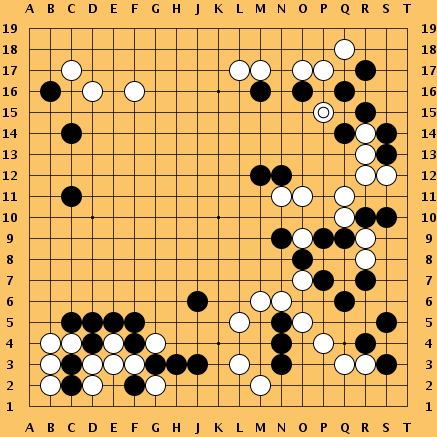
\includegraphics[width=0.25\linewidth]{goboard}
\end{center}
\caption{a snapshot of the Go board}
\label{fig:goboard}
\end{figure}

\begin{figure}[H]
\centering
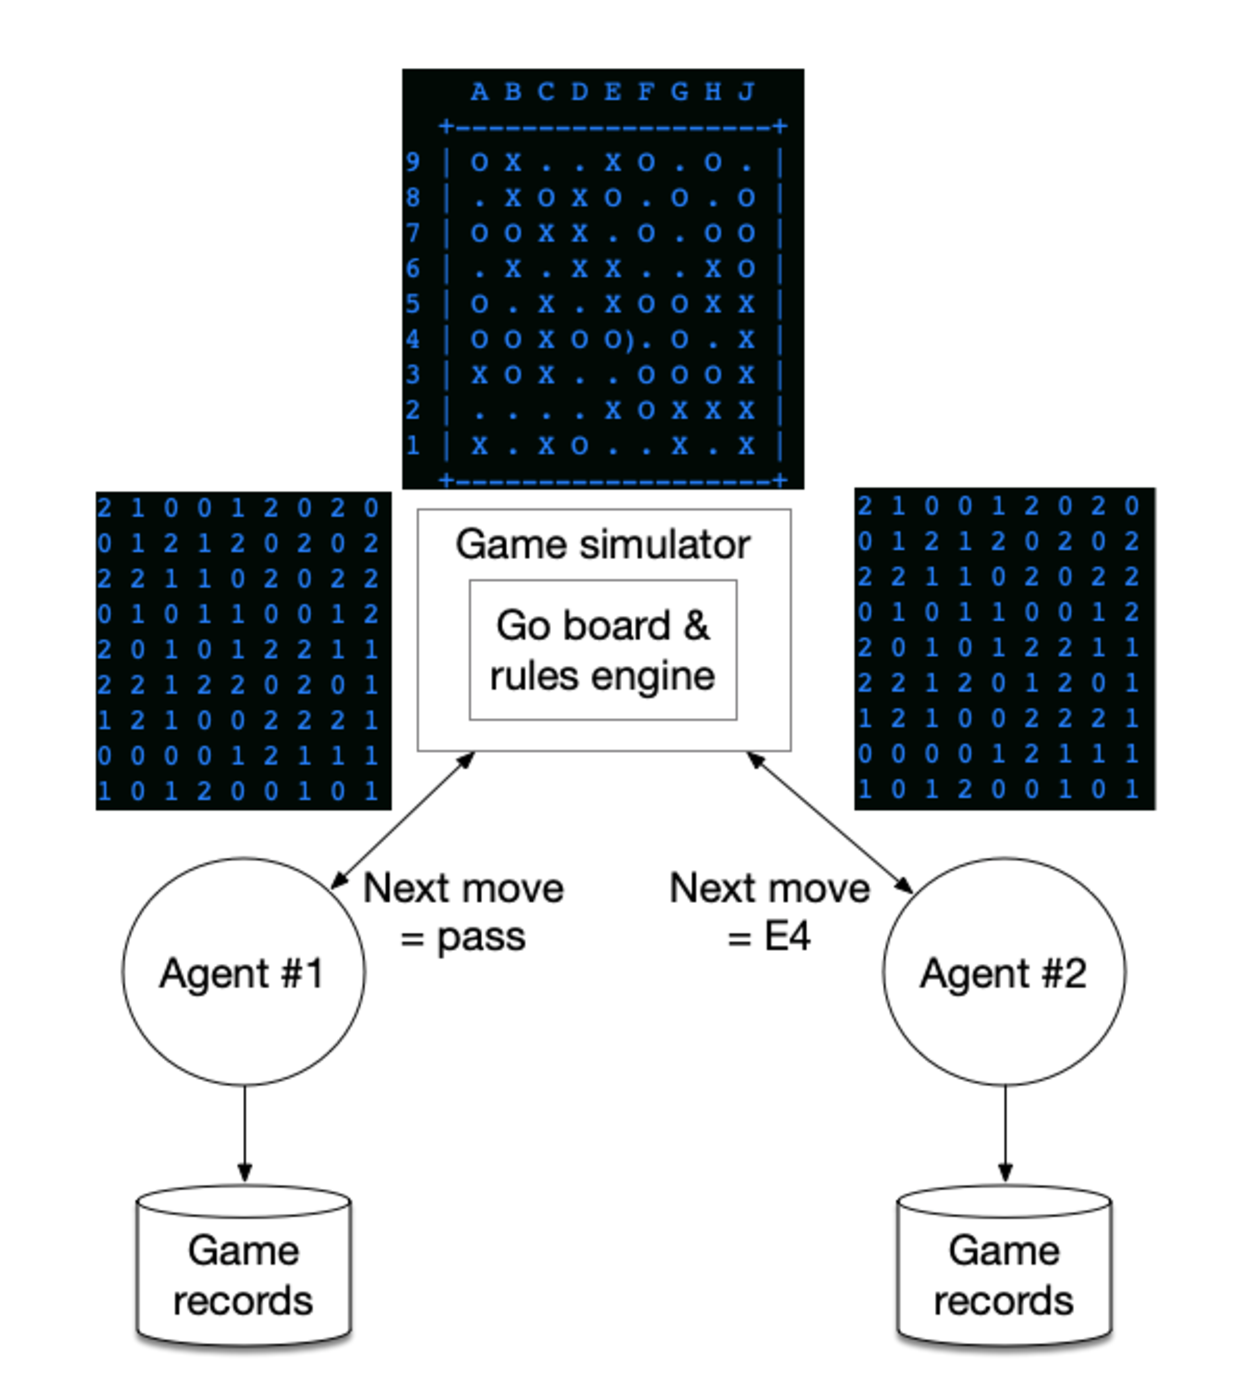
\includegraphics[width=0.8\linewidth]{simulator}
\caption{Environment setup. For Go boards drawn in all the figures, 'x' represents black stone and 'o' represents white stone. For numpy arrays, '0' means empty, '1' represent black stone and '2' represents white stone. All examples assume $9 \times 9$ board.}
\label{fig:env}
\end{figure}

\begin{figure}
\centering
\includegraphics[width=1.0\linewidth]{mctsselect}
\caption{MCTS node selection via tree policy: shows 4 successor states only for brevity. $a=67$ is selected. $n, q$ is visit count and value for each node respectively. $a=76$ has more visit counts but lower value.}
\label{fig:mctsselect}
\end{figure}

\begin{figure}
\centering
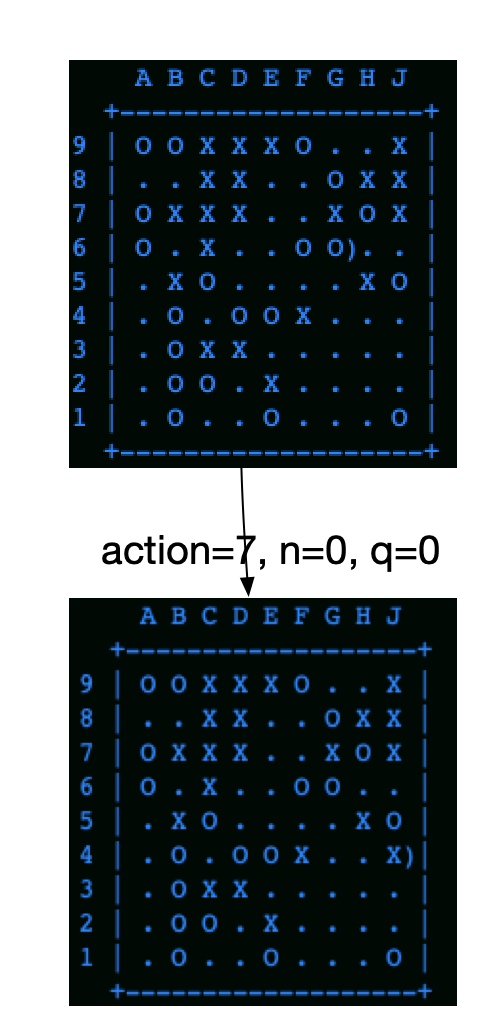
\includegraphics[width=0.3\linewidth]{mctsexpand}
\caption{A new node $\text{Succ}(s, a=7)$, randomly chosen, is expanded with zero visit count and value. }
\label{fig:mctsexpand}
\end{figure}

\begin{figure}
\centering
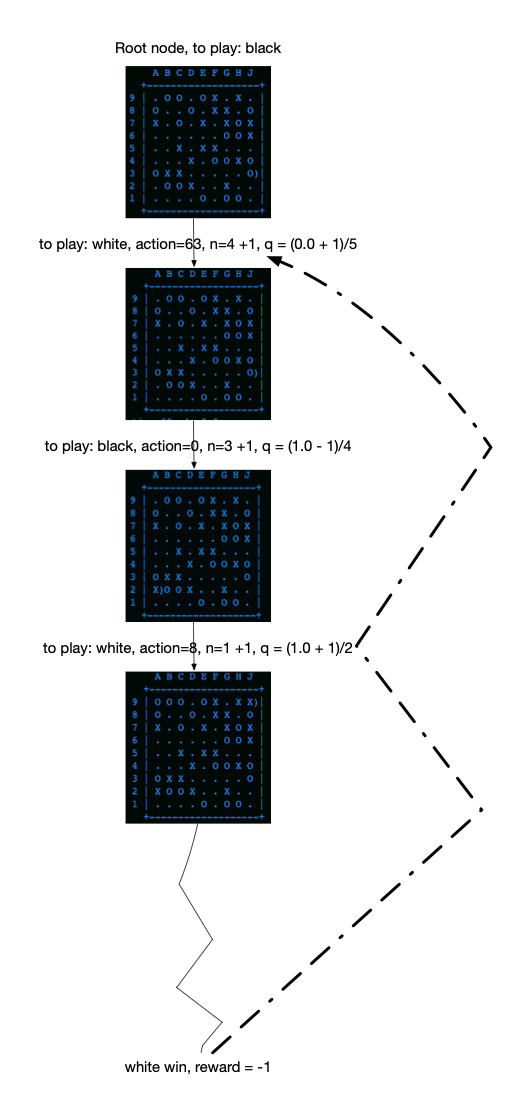
\includegraphics[width=0.7\linewidth]{mctsbackup}
\caption{After the simulation is done. The result is backed up to all nodes on the path. Note the reward is from black player's perspective and needs to be adjusted for white player.}
\label{fig:mctsbackup}

\end{figure}
\begin{figure}
\centering
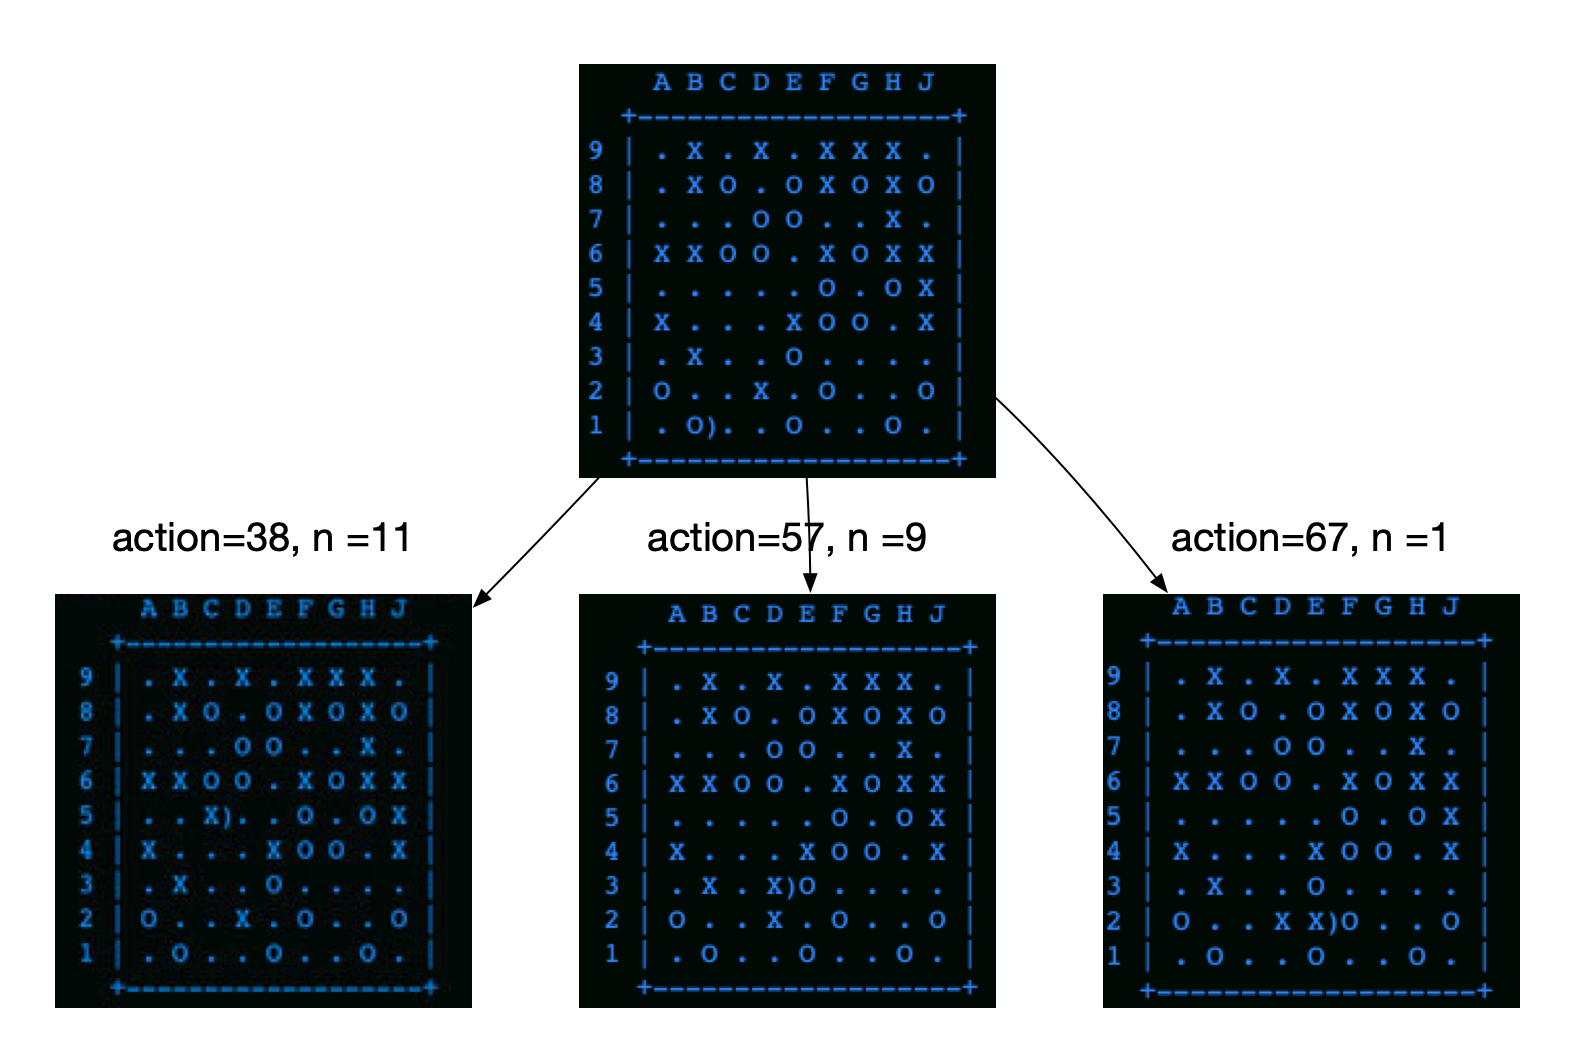
\includegraphics[width=0.9\linewidth]{mctsfinal}
\caption{After all rollout are done. Select the next move with maximum moves. Shows 3 successor states from root state only. The action $a=38$ is selected.}
\label{fig:mctsfinal}
\end{figure}

\begin{figure}
\centering
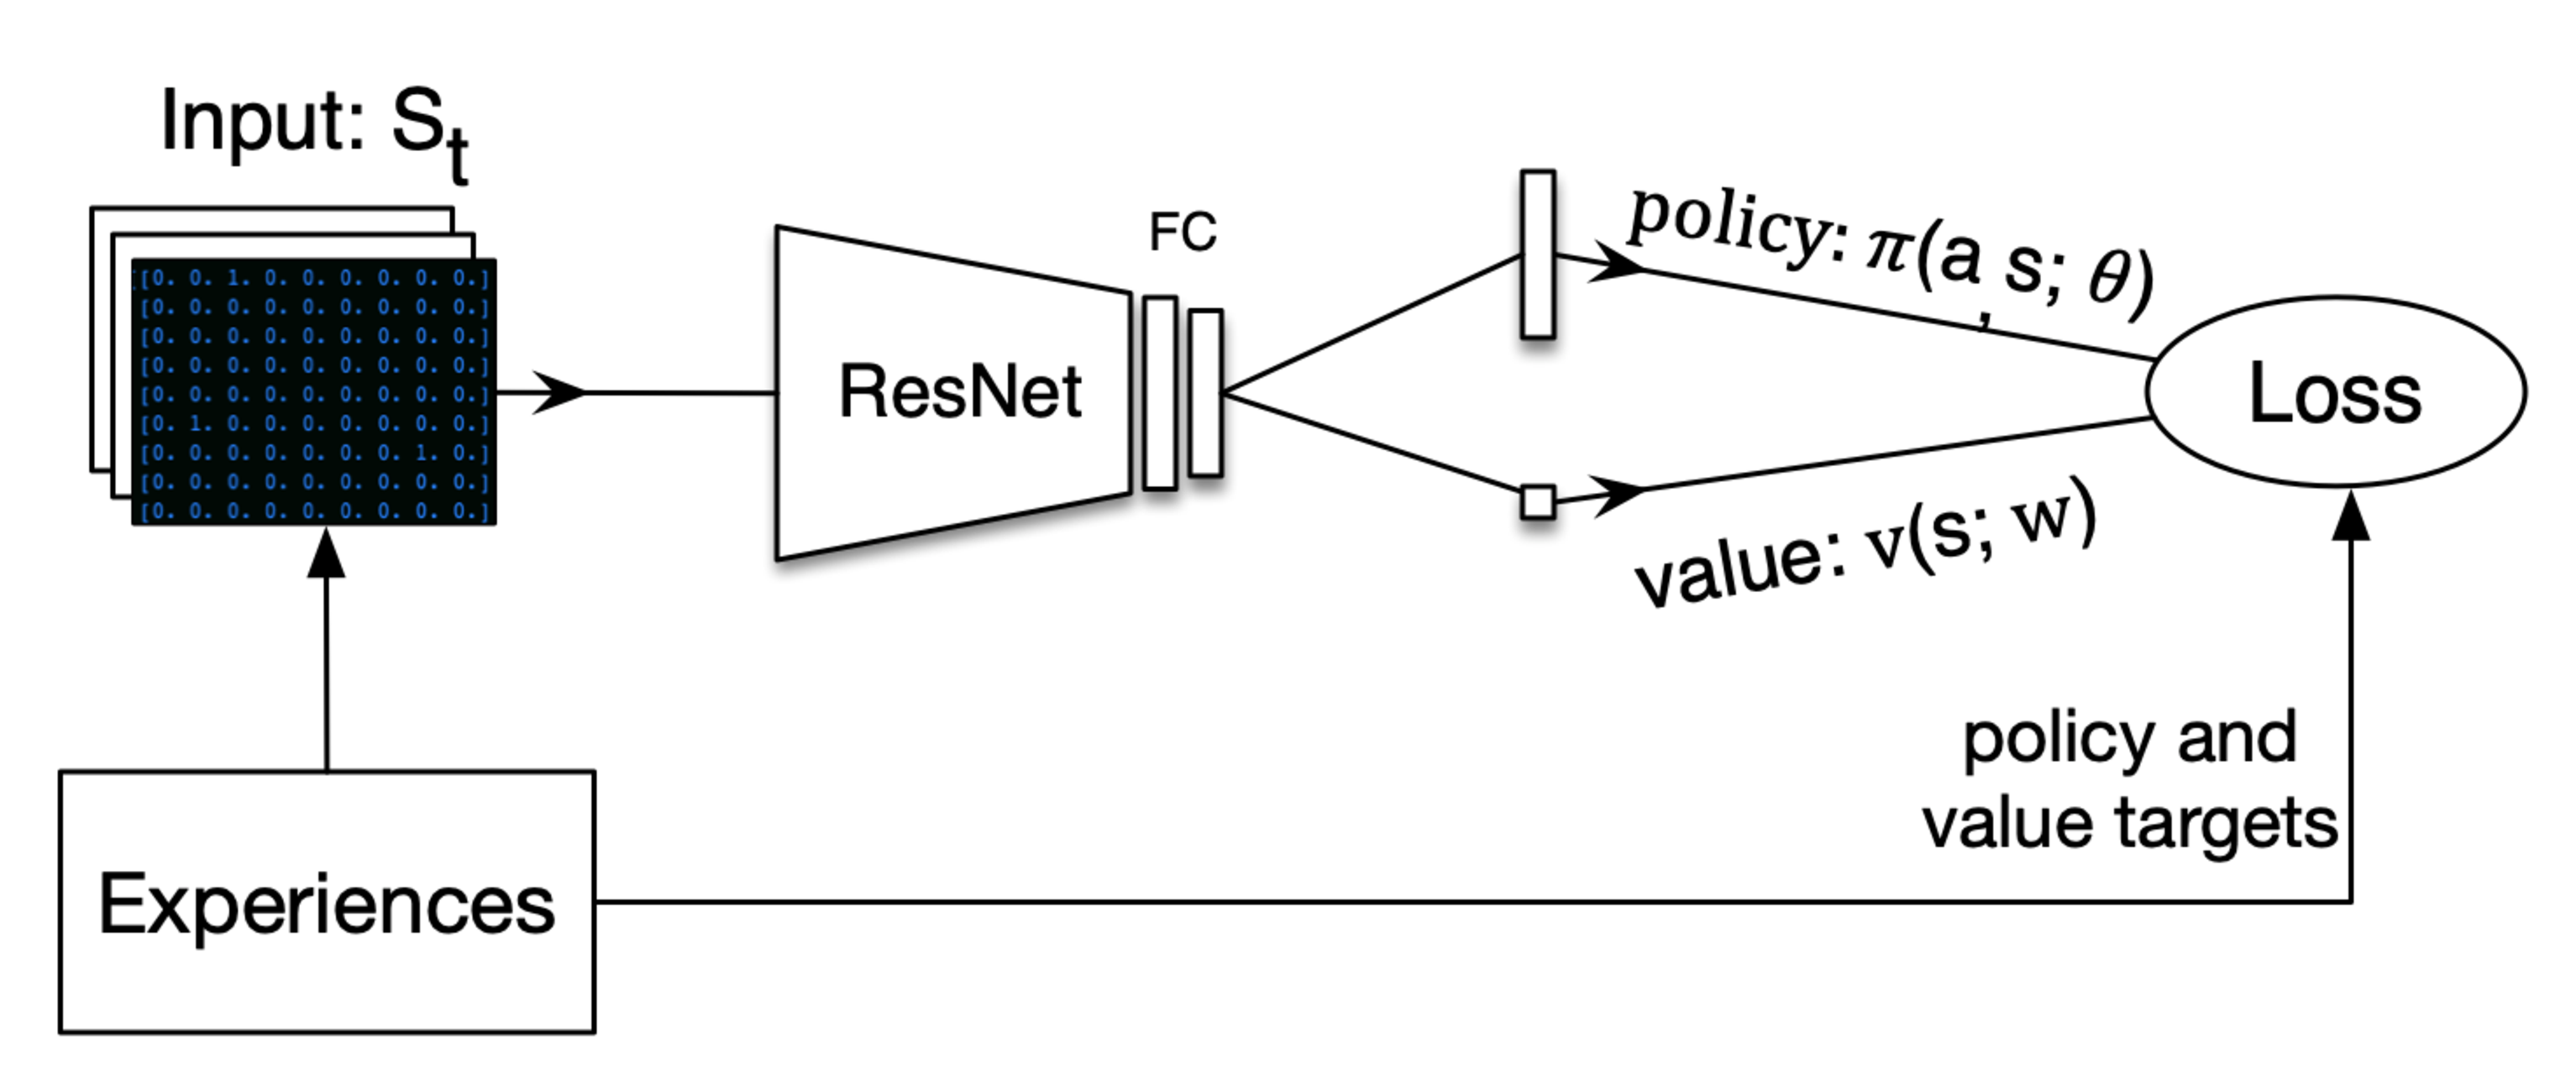
\includegraphics[width=0.8\linewidth]{nn}
\caption{network architecture for policy gradients and NN guided MCTS approaches. The features and policy/value targets are gathered from self-play experiences. FC stands for Fully Connected layer. Features, targets and Loss are discussed in details in text.}
\label{fig:nn}
\end{figure}

\begin{figure}
\centering
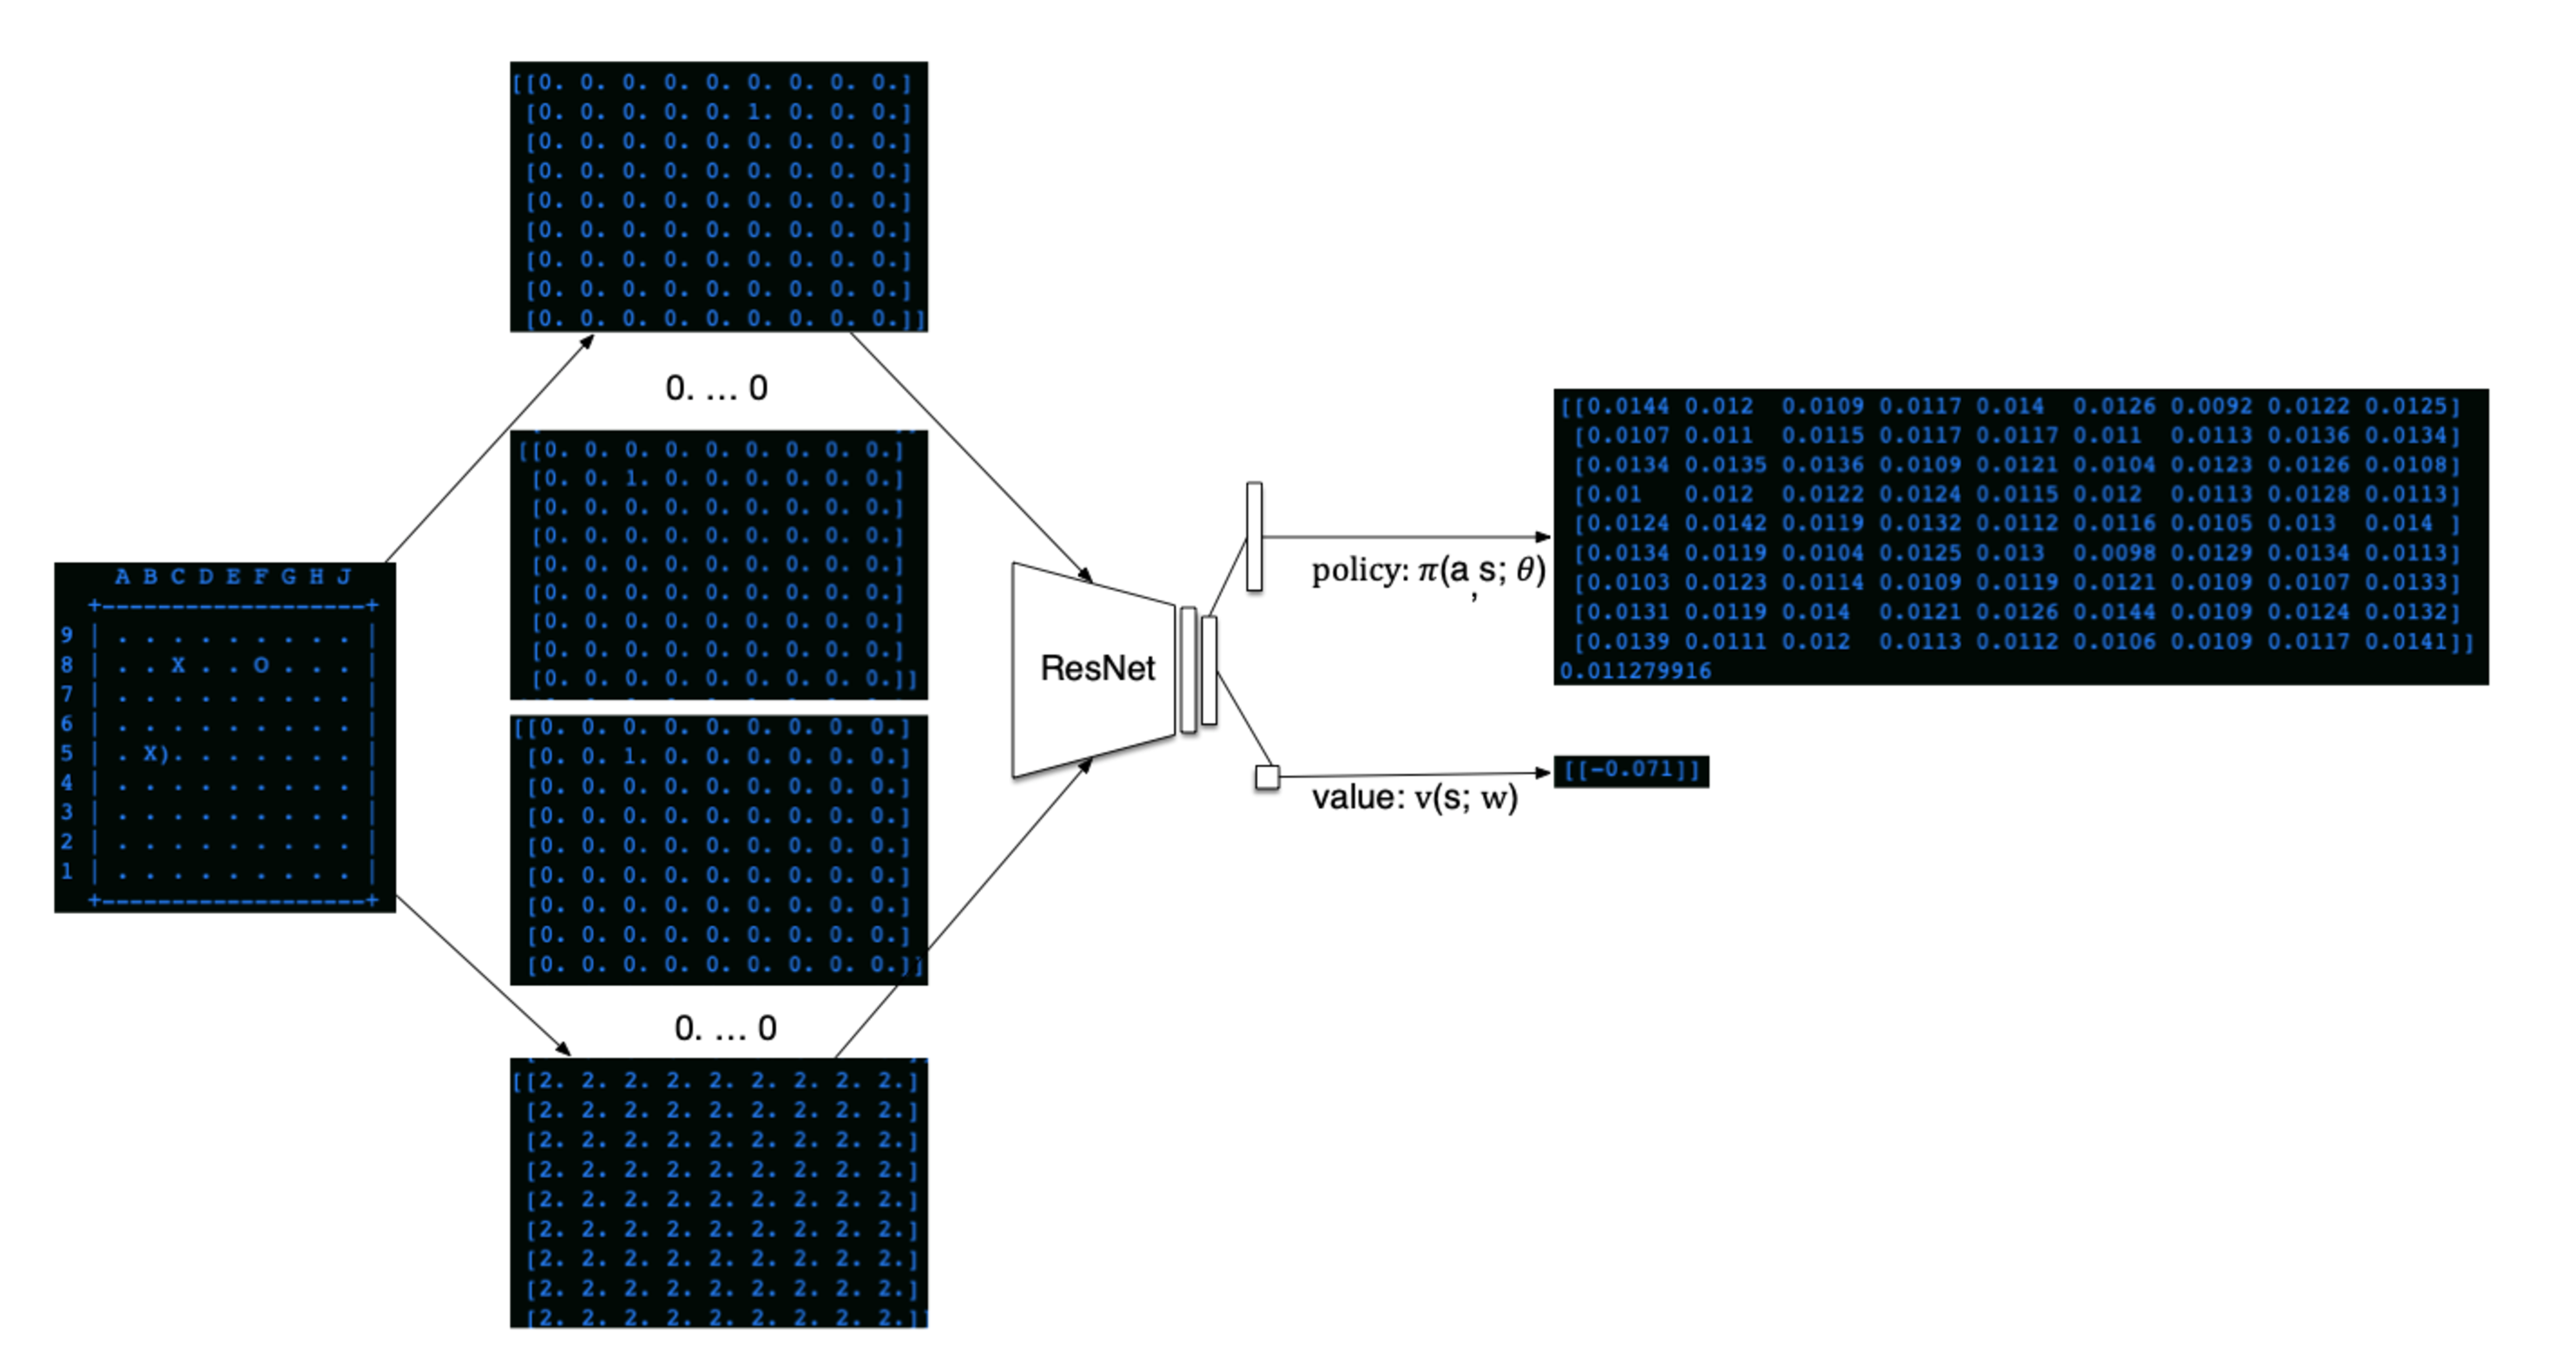
\includegraphics[width=1.0\linewidth]{inference}
\caption{example for an input/output for neural network. The input is $17 \times 9 \times 9 $ arrays, created from the board position. There are two outputs, one $82$-tuple of probability vector $\pi_{\theta}$ and one scalar $v_w \in [-1, 1]$. Refer to the text for more details. }
\label{fig:inference}
\end{figure}

\begin{table}[ht]
  \caption{Neural Network Architecture}
  \label{tbl:nna}
  \centering
  \begin{tabular}{c | c | c | c}
    Number & Layer description    & Layer input \\
    \hline
    1 & Input layer                                           & N/A \\                      
    2 & Conv2D 32 $3 \times 3$ filters with batch normalization and ReLU activation & 1\\
    3 & Conv2D 32 $3 \times 3$ filters with batch normalization and ReLU activation & 2\\
    4 & Conv2D 32 $3 \times 3$ filters with batch normalization                     & 3 \\
    5 & Add and then ReLU activation                                               & 2 \& 4 \\
    \ldots & repeated (3,4,5) 7 times & \ldots    \\
    27 & Conv2D 32 $3 \times 3$ filters, batch normalization and ReLU activation & 26 \\
    28 & Conv2D 32 $3 \times 3$ filters, batch normalization                     & 27 \\
    29 & Add and then ReLU activation                                               & 26 \& 28 \\
    \hline
    30 & Conv2D 2 $1 \times 1$ filters, batch normalization and ReLU activation & 29 \\
    31 & policy output, dense layer $162 \times 83$ with Softmax activation & 30 \\
    \hline
    32 & Conv2D 1 $1 \times 1$ filters, batch normalization and ReLU activation & 29 \\
    33 & hidden layer, dense layer $128 \times 81$ & 31 \\
    34 & value output, scalar, dense layer $81 \times 1$ & 31 \\
    \hline
  \end{tabular}
\end{table}
\end{document}
